\documentclass{beamer}
\usetheme{Boadilla}
\usepackage{color}
\newcommand{\wf}{\color{white}}
\newcommand{\tf}{\color{black}}
\begin{document}
\title{Effizienz der gerechten Aufteilung von beliebig teilbaren G\"utern}  
\author{Alina Elterman}
\date{\today}  

\frame{\titlepage} 

\frame{\frametitle{Inhaltsverzeichnis}\tableofcontents} 


\section{Einleitung} 
\frame{\frametitle{Cake-Cutting} 
 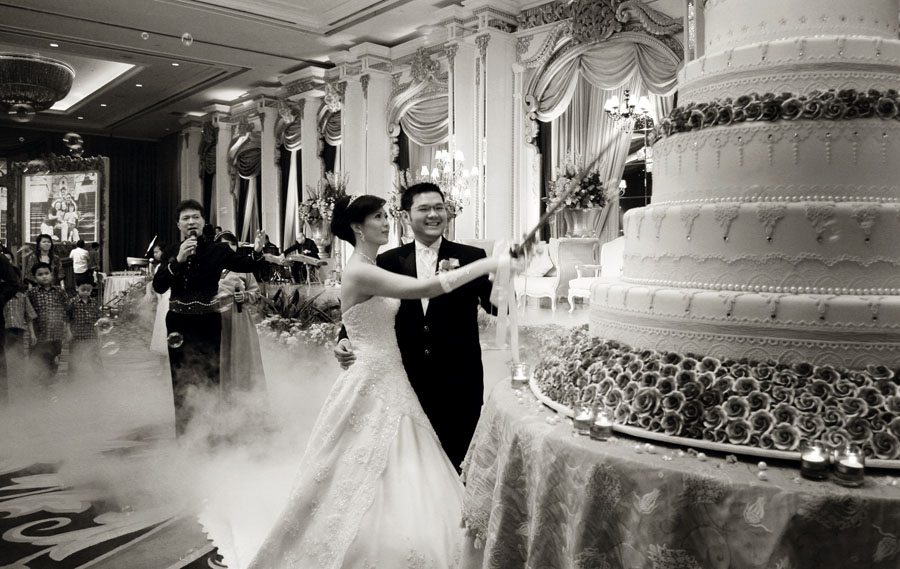
\includegraphics[height=7cm]{Grosseer.jpg} \pause
\newline
Kuchen - Metapher f\"ur ein beliebig oft teilbares Gut
}

\frame{\frametitle{Cake-Cutting} 
 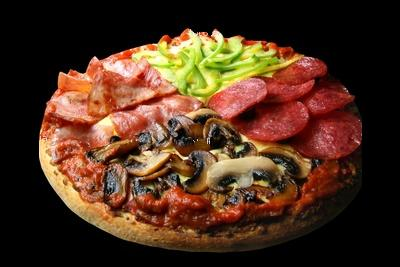
\includegraphics[height=7cm]{4j.jpg}\pause
\newline
Die Pr\"aferenzen auf bestimmte St\"ucke k\"onnen sich unterscheiden! 
}

\section{Grundbegriffe} 
\subsection{Der Kuchen und die Bewertung}
\frame{\frametitle{Grundbegriffe}
\begin{itemize}
\item $P_n$=$\{p_1,...,p_n\}$ - Menge von $n$ Spieler
\item Intervall $X=[0,1]$ - einziges, heterogenes, beliebig teilbares Gut (Kuchen) 
\item$v_i:\{X'|X'\subseteq X\}\mapsto [0,1]$ - Bewertungsfunktion des Spielers $p_i$ mit bestimmten Eigenschaften
\item $X_i$ ist das St\"uck vom Spieler $p_i$ bei oder nach der Aufteilung und $v_i(X_i)$ seine Bewertung oder sein Nutzwert
\end{itemize} 

}
\frame{\frametitle{Gerechtigkeitskriterien}
\begin{itemize} 
\item{\textbf{Proportionalit\"at}
\newline Eine Aufteilung ist \underline{proportional}, falls  $v_i(X_i) \geq 1/n$ f\"ur jeden Spieler $p_i \in P_N$ gilt.}
\item{\textbf{Neidfreiheit}
\newline Eine Aufteilung ist \underline{neidfrei}, falls $v_i(X_i) \geq v_i(X_j)$ f\"ur jedes Paar von Spielern $p_i, p_j \in P_N$.} 
\item{\textbf{Exaktheit}
\newline Eine Aufteilung ist \underline{exakt}, falls $v_i(X_i) = v_j(X_j)$ f\"ur jedes Paar von Spielern $p_i, p_j \in P_N$.}
\end{itemize}
}
\frame{\frametitle{Effizienz}
\"Ublicherweise:
\newline Eine Aufteilung ist \underline{effizient (Pareto optimal)}, falls keine andere Aufteilung existiert, die einem Spieler ein von ihm besser bewertetes St\"uck einbringt, ohne die Situation eines anderen Spielers zu verschlechtern.\\\pause
\wf srgndf\\
\tf
Hier: \textbf{Effizienz} = Grad der Zufriedenheit aller Spieler = $\sum_{i=1}^n{v_i(X_i)}$.\\
}

\frame{\frametitle{Soziales Wohl}
Eine Aufteilung ist \underline{optimal}, falls sie die Summe der Nutzwerte von allen Spielern maximiert.\\
}

\frame{\frametitle{\"Ubersicht \"uber Cake-Cutting}
\begin{itemize}
\item Entwicklung und Analyse von gerechten Protokollen
\item Existenzbeweise von gerechten Aufteilungen
\item Approximationsalgorithmen der gerechten Aufteilung
\end{itemize}
}

\frame{\frametitle{\"Ubersicht \"uber Cake-Cutting}
Was wurde noch nicht erforscht?\\
\wf khfbks \\
\wf kbrfkd \\
\wf 
\huge{Effizienz bei Protokollen!}
}

\frame{\frametitle{\"Ubersicht \"uber Cake-Cutting}
Was wurde noch nicht erforscht?\\
\wf khfbks \\
\wf kbrfkd \\
\tf 
\huge{Effizienz bei Protokollen!}
}

\section{Der Preis der Gerechtigkeit}
\frame{\frametitle{Der Preis der Gerechtigkeit}
\begin{figure}[!h]
\centering
 
\includegraphics[height=7cm]{pr.jpg}
\end{figure}
}
\frame{\frametitle{Der Preis der Gerechtigkeit}
Wie viel Effizienz muss aufgegeben werden f\"ur die Gerechtigkeit?\\
\begin{tabular}{rr}
&\\
&\\
Verh\"altnis :& \underline{Gr\"osste m\"ogliche Nutzwert}\\
&{Nutzwert im besten gerechtesten Fall }\\
\end{tabular}
}
\subsection{Preis der Proportionalit\"at und Neidfreiheit f\"ur $n=2$}
\frame{\frametitle{Preis der Proportionalit\"at und Neidfreiheit f\"ur $n=2$}
Sei $\mathcal{O}$ eine optimale Aufteilung und $\mathcal{E}$ die effizienteste proportionale Aufteilung.
Sei $A,B,C$ und $D$ eine Partitionierung des Kuchens mit folgenden Eigenschaften:\\\pause
\begin{itemize}
\item $A$ wird in $\mathcal{O}$ und $\mathcal{E}$ Spieler $p_1$ zugeordnet
\item $B$ wird in $\mathcal{O}$ und $\mathcal{E}$ Spieler $p_2$ zugeordnet
\item $C$ wird in $\mathcal{O}$ Spieler $p_1$  und in $\mathcal{E}$ Spieler $p_2$ zugeordnet
\item $D$ wird in $\mathcal{O}$ Spieler $p_2$  und in $\mathcal{E}$ Spieler $p_1$ zugeordnet\pause
\end{itemize}
Es gilt $v_1(A)\geq v_2(A)$, $v_1(B)\leq v_2(B)$, $v_1(C)\geq v_2(C)$ und $v_1(D)\leq v_2(D)$.
}

\frame{\frametitle{Preis der Proportionalit\"at und Neidfreiheit f\"ur $n=2$}
Betrachte $v_1(C) >v_2(C)$ und $v_1(D) = v_2(D) = 0$:\\\pause
Es gibt ein $X_c\subseteq C$ mit  $v_1(X_c)=x$ und $v_2(X_c)=x*v_2(C)/v_1(C)$ und damit $v_1(X_c) \geq v_2(X_c)$!
Analog f\"ur $D$ und $X_d$.\\\pause Damit bleibt die Aufteilung $v_1(A+X_c+D-X_d)$ und $v_2(B+X_d+C-X_c)$ proportional, hat aber einen gr\"osseren Nutzwert als $\mathcal{E}$.\\\pause
Es gilt: $v_2(A)=1/2$ und $v_2(A)/v_1(A)\leq v_2(C)/v_1(C)$.\\\pause
Damit folgt die Absch\"atzung:\\
\wf ekbfrkj\\ \tf
$\frac{v_1(A)+v_2(B)+v_1(C)}{v_1(A)+v_2(B)+v_2(C)}$$\leq$$\frac{v_1(A)+1/2+(1-v_1(A))(1-1/{2v_1(A)})}{v_1(A)+1/2}$\\
\wf hkbfraiegfb\\\tf
Das Maximum ist $8-4\sqrt{3}$ f\"ur $v_1(A)=\frac{1+\sqrt{3}}{4}$.\\\pause
\wf ekbfkerhbf \\\tf
Bsp: $v_1(A)=1$, $v_1(B)=0$, $v_2(A)=\sqrt{3}-1$ und $v_2(B)=2-\sqrt{3}$.

}

\subsection{Zusammenfassung}
\frame{\frametitle{Resultate von I. Caragiannis, C. Kaklamanis, P. Kanellopoulos und M. Kyropoulou}
$\begin{tabular}{rrrr}
\begin{tabular}{|r|}
\hline
\\
\hline
Preis der\\
\hline Proportionalit\"at\\
\hline
Neidfreiheit\\
\hline
Exaktheit\\
\hline
\end{tabular}
\begin{tabular}{|r|}
\hline
Untere Schranke\\
\hline
\\
\hline
$\Omega(\sqrt{n})$\\
\hline
$\Omega(\sqrt{n})$\\
\hline
$(n+1)^2/{4n}$\\
\hline
\end{tabular}
\begin{tabular}{|r|}
\hline
Obere Schranke\\
\hline
\\
\hline
$\mathcal{O}(\sqrt{n})$\\
\hline
$n-1/2$\\
\hline
$n$\\
\hline
\end{tabular}
\begin{tabular}{|r|}
\hline
$n=2$\\
\hline
\\
\hline
$8-4 \sqrt{3}$\\
\hline
$8-4 \sqrt{3}$\\
\hline
$9/8$\\
\hline
\end{tabular}
\end{tabular}$
}

\section{Vorschau und offene Fragen}
\frame{\frametitle{N\"achstes Mal:}
\begin{itemize}
\item Utilitarismus und Egalitarismus
\item Preis der Effizienz (R\"uckrichtung)
\item Zusammenh\"angende St\"ucke
\end{itemize}
}
\frame{\frametitle{Fragen:}
\begin{itemize}
\item Gibt es immer eine effiziente Aufteilung?
\item L\"asst sich Gerechtigkeit und Effizienz immer vereinigen?
\item Wie sehen effiziente Protokolle aus?
\end{itemize}
}

\frame{\frametitle{}
 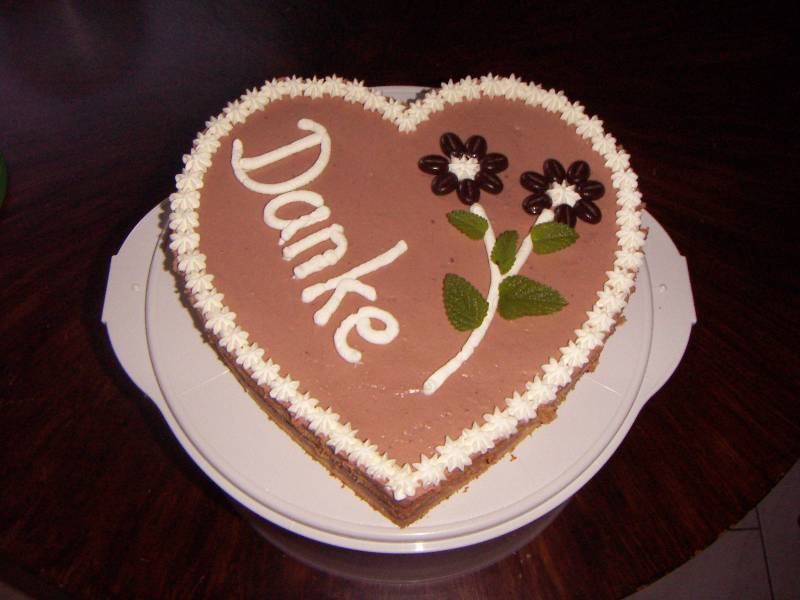
\includegraphics[height=8cm]{Danke.jpg}\\
F\"ur die Aufmerksamkeit!
}


\section{Quellenverzeichnis}
\frame{\frametitle{Quelle:}[CKKK09] I. Caragiannis, C. Kaklamanis, P. Kanellopoulos und M. Kyropoulou: The Efficiency of Fair Division. \emph{WINE '09 Proceedings of the 5th International Workshop on Internet and Network Economics}, 475 - 482, 2009.
}
\end{document}

